\chapter{緒論}
\label{c:intro}

近年來,隨著網際網路的快速發展,網際網路中開始出現越來越多彙整人類知識的網站與資源,
如Wikipedia、Freebase等,是透過來自世界各地的志願編輯者一字一句的貢獻建立而成的。

但這種形式的知識僅有人類可以利用,為了讓計算機可以利用人類的知識來輔助、改善人工智慧、資料截取、知識汲取、自動問答系統等任務,
便需要計算機可以理解的結構化知識,於是,便有了透過擷取Wikipedia等網站資訊,建構結構化知識的資源如YAGO、DBpedia。

% FIXME TODO - 說明能夠快速抓住變動的知識是很重要的
% TODO - 可能可以加上 Linked-Data 的圖片

% 知識庫不會憑空產生,多半是擷取人工編輯的成果或靠人工編輯,因此如何讓人工編輯的速度可以跟上知識產生的速度便成為一個重要的課題。

\section{背景介紹}
% Keyword: 知識庫、內容串流
% FIXME
如Wikipedia、Freebase、YAGO、DBpedia等這類儲存記錄實體(Entity)與實體之特性(Properties)、關係(Relationships)的資料庫被稱為知識庫(Knoledge Base)。
以Wikipedia來說,Wikipedia以文章的形式儲存了人物、公司、組織、事件等實體,以超連結(Hyperlink)連結文章與文章的文句則可視為一種關係的描述,
例如「\zhbf{甲}是\zhbf{乙}的員工」這樣的句子;而文章中的資訊框(Infoboxes)則是一種對實體之特性半結構化(Semi-structured)的描述。    
%TODO - 加圖片(從KBA Background)

而知識庫的維護者,如Wikipedia的志願編輯者,人數比起知識庫中的實體實在是非常的少,
這意味著當舊有的知識產生變化時,或有新的知識出現時,這樣的變動或新增需要經過一段長時間後,編輯者才會更新知識庫。\cite{Nakashole:2012:PATTY}

為了縮短新知識產生到更新知識庫的這段差距,自2012年起至今的每年NIST的TREC(Text Retriveal Conference)都會舉辦KBA(Knowledge Base Acceleration)競賽,
提供一個有4973小時,每個小時包含100000篇文件的的內容串流(Content Stream),模擬現實世界之中不斷產生的新文章,包含了新聞、部落格、論壇等。
並給定了一組關注的實體,包含了人物、組織或建築,希望參賽者可以建立一個系統過濾內容串流中的資訊,
推薦編輯者哪些資訊可以幫助編輯者更新知識庫中關於這些目標實體的知識。
%TODO - Add KBA overview's image


\section{研究動機}
% Keyword: 知識庫加速
% TODO




\section{研究目標}
% Keyword: given a content stream, 回答有沒有某個特性這樣
% TODO

\section{論文架構}  % TODO FIXME
本論文共分成五個章節。
第一章是緒論,簡介本研究的背景、動機與目標。
第二章是文獻探討,列舉了一些相關的研究與資源。
第三章是研究方法,提出如何於內容串流中究偵測實體特性的方法與步驟。
第四章是實驗結果與分析,
第五章是結論與未來展望,

%\begin{figure}
%\centering
%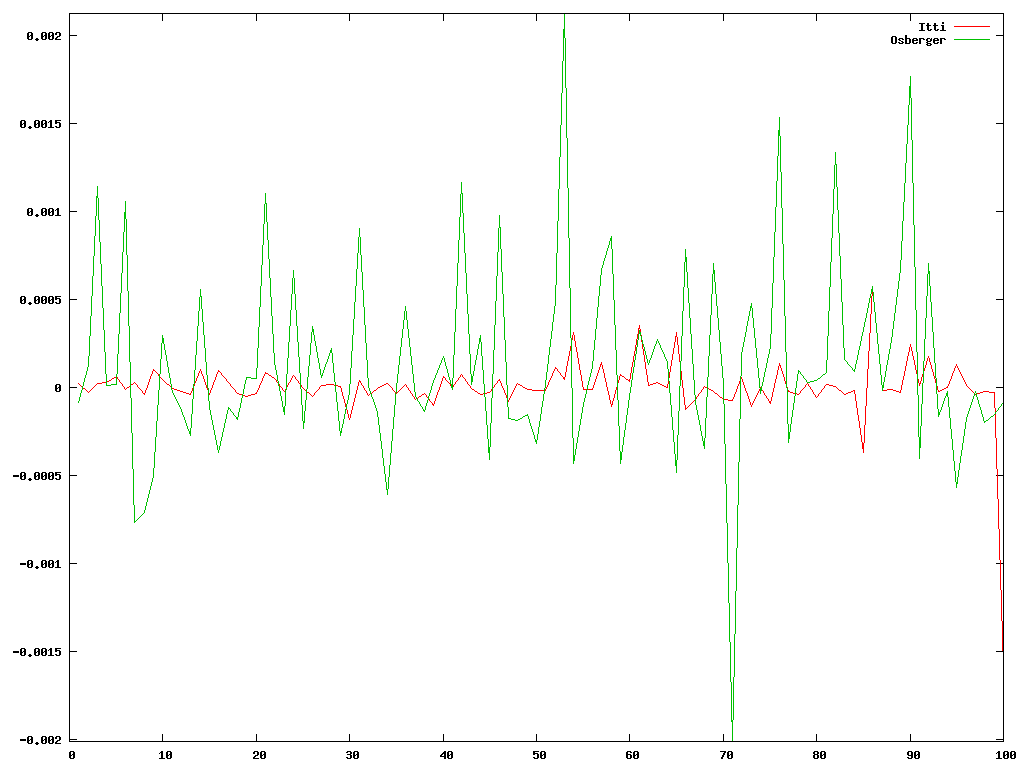
\includegraphics[width=0.45\textwidth]{images/kl}
%\caption{kl-distance}
%\label{kl}
%\end{figure}

%\begin{table}[t]
%\begin{center}
%\begin{tabular}{lcc}
%
%\hline
%                    &  {\small Itti's method}     & {\small Fuzzy growing}    \\
%\hline
%{\small Precision}           &  0.4475    & 0.4506 \\
%{\small Recall}              &  0.5515    & 0.5542 \\
%\hline
%
%\end{tabular}
%\caption[Evaluation of FOA sets]{\small Evaluation of FOA sets. } \label{t:FOA}
%\end{center}
%\end{table}

